\begin{statementbox}
\textbf{先说它解决什么问题。} 当题目出现取整符号时，关键不是四舍五入，而是先分清“整数部分”和“小数部分”，再把取整条件改写成普通不等式。

\textbf{结论一｜整数部分的定义。} 对任意 $x\in\mathbb R$，$\lfloor x\rfloor$ 表示\textbf{不超过 $x$ 的最大整数}，称为 $x$ 的整数部分，教材也记作 $[x]$。对任意 $n\in\mathbb Z$，
\[\boxed{\lfloor x\rfloor=n\iff n\le x<n+1.}\]
因此
\[x-1<\lfloor x\rfloor\le x.\]
定义域为 $\mathbb R$，值域为 $\mathbb Z$，在实数集上单调不减，图像是左闭右开的台阶型。
\begin{center}
\begin{tikzpicture}[scale=0.92]
\draw[->] (-3.6,0)--(3.6,0) node[right]{$x$};
\draw[->] (0,-3.2)--(0,3.4) node[above]{$y$};
\foreach \n in {-3,-2,-1,0,1,2,3}{\draw (\n,0.08)--(\n,-0.08) node[below,font=\scriptsize]{$\n$};}
\foreach \n in {-3,-2,-1,0,1,2}{
  \draw[teal!70!black,very thick] (\n,\n)--(\n+1,\n);
  \fill[teal!70!black] (\n,\n) circle(1.8pt);
  \draw[teal!70!black,fill=white] (\n+1,\n) circle(1.8pt);
}
\node[above right,font=\small] at (1.4,2.0) {$y=\lfloor x\rfloor$};
\end{tikzpicture}
\end{center}


\textbf{结论二｜小数部分的定义。} 定义
\[\boxed{\{x\}=x-\lfloor x\rfloor.}\]
称 $\{x\}$ 为 $x$ 的小数部分。由 $n\le x<n+1$ 两边减去 $n$，可知
\[\boxed{0\le \{x\}<1.}\]
于是任意实数都能唯一写成 $x=\lfloor x\rfloor+\{x\}$。在 $[n,n+1)$ 上，整数部分恒为 $n$，小数部分为 $x-n$。小数部分函数的定义域为 $\mathbb R$，值域为 $[0,1)$，并满足 $\{x+1\}=\{x\}$，所以图像以 $1$ 为最小正周期重复出现。
\begin{center}
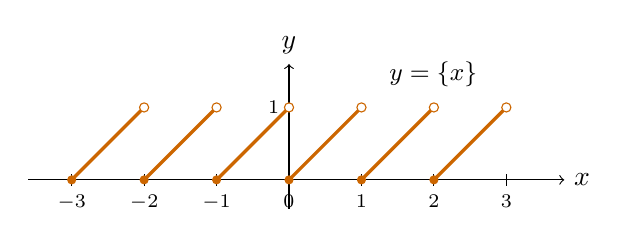
\begin{tikzpicture}[scale=0.92]
\draw[->] (-3.6,0)--(3.8,0) node[right]{$x$};
\draw[->] (0,-0.4)--(0,1.6) node[above]{$y$};
\foreach \n in {-3,-2,-1,0,1,2,3}{\draw (\n,0.08)--(\n,-0.08) node[below,font=\scriptsize]{$\n$};}
\draw (0,1) node[left,font=\scriptsize]{$1$};
\foreach \n in {-3,-2,-1,0,1,2}{
  \draw[orange!80!black,very thick] (\n,0)--(\n+1,1);
  \fill[orange!80!black] (\n,0) circle(1.8pt);
  \draw[orange!80!black,fill=white] (\n+1,1) circle(1.8pt);
}
\node[above right,font=\small] at (1.25,1.15) {$y=\{x\}$};
\end{tikzpicture}
\end{center}


\textbf{结论三｜整数边界不等式。} 前两条结论说明，取整的实质是确定 $x$ 所属的单位区间。比较取整值与整数 $n$，就只需比较 $x$ 与区间边界。对 $n\in\mathbb Z$，
\[\begin{aligned}
\lfloor x\rfloor\ge n&\iff x\ge n,\\
\lfloor x\rfloor<n&\iff x<n,\\
\lfloor x\rfloor\le n&\iff x<n+1,\\
\lfloor x\rfloor>n&\iff x\ge n+1.
\end{aligned}\]

\textbf{结论四｜整数平移与加法。}
\[\boxed{\lfloor x+m\rfloor=\lfloor x\rfloor+m\quad(m\in\mathbb Z).}\]
\[\lfloor x\rfloor+\lfloor-x\rfloor=\begin{cases}0,&x\in\mathbb Z,\\-1,&x\notin\mathbb Z.\end{cases}\]
\[\boxed{\lfloor x\rfloor+\lfloor y\rfloor\le\lfloor x+y\rfloor\le\lfloor x\rfloor+\lfloor y\rfloor+1.}\]
当且仅当 $\{x\}+\{y\}\ge1$ 时，加法结果比两次取整的和大 $1$。
\end{statementbox}
